\chapter{Background}
\label{cp:Background}

\begin{comment}
Please write down the basic background for your research, e.g., the fundamental concepts of the approaches that you use in the thesis, so that other people (who do not have the background) can understand your work.

Here is one example for sigmoid function:

The sigmoid function is defined by formula~\ref{eq:sigmoid}. It can compress the input into the interval $(0, 1)$. The drawback of the sigmoid activation function is the so-called ``kill gradients'': if the input values locate in the tail of 0 or 1, the gradient at these regions tend to be zero. If the sigmoid function is used multiple times in a neural network, the gradients may be very small or even disappear.

\begin{equation}
\label{eq:sigmoid}
\centering{f(x) = \frac{1}{1 + e^{-x}}}.
\end{equation}
\end{comment}

\section{Discrete wavelet decomposition}


\section{Control chart}

It is well known that statistical process control (SPC) is a
powerful tool to prevent production of defects and
nonconforming products. . Researchers believe that control charts are the
most featured tool of SPC. Control charts can be classified
into 2 categories of univariate and multivariate charts. In
univariate control charts, . However, in multivariate control charts, one is
interested in monitoring simultaneous changes in the parameter
vector of an underlying multivariate distribution over time.


Statistical process control (SPC) is a powerful collection of problem-solving
tools useful in achieving process stability and improving capability through the reduction of variability.
SPC is one of the greatest technological developments of the twentieth century because it is based on sound underlying principles, is easy to use, has significant impact, and can be applied to any process~\cite{montgomery2020introduction}. Its seven major tools are
\begin{enumerate}
    \item Histogram or stem-and-leaf plot
    \item Check sheet
    \item Pareto chart
    \item Cause-and-effect diagram
    \item Defect concentration diagram
    \item Scatter diagram
    \item Control chart
\end{enumerate}

Of this seven tools, Control chart is probably the easiest yet effective tool to analyze the process stability. To best understand the concepts of Control chart, the classification of Control chart need to be clarified. Depending on the number of process characteristics to be monitored, there are two basic types of control charts. The first, referred to as a univariate control chart, is a graphical chart of one quality characteristic, in which one is interested in monitoring
changes in the parameter of an underlying univariate distribution
over time. The second is a multivariate control chart, which is a graphical chart of a statistic that fuses more than one quality characteristic to monitor simultaneous changes in the parameter
vector of an underlying multivariate distribution over time.


More specificlly, the control chart is a graphical display, which plots the value of the quality characteristic that has been measured or calculated from a sample versus the sample number or versus time. Normally there are three lines in a control chart: a center line that correspond to the mean value for the in-control process. Two other horizontal lines, called the upper control limit (UCL) and the lower control limit (LCL). These control limits are chosen so that almost all of the data points will fall within these limits as long as the process remains in-control. A typical control chart is shown in Fig.~\ref{fig:control_chart}.

\begin{figure}[h]
\centering
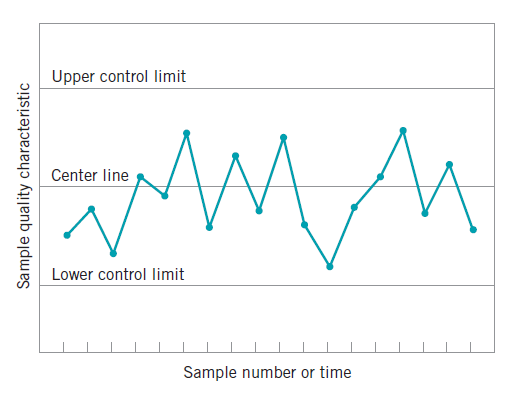
\includegraphics[width=1\textwidth]{images/control_chart.PNG}
\caption[A typical control chart.]{a center line that correspond to the mean value for the in-control process. Two other horizontal lines, called the upper control limit (UCL) and the lower control limit (LCL). Figure is adapted from ~\cite{montgomery2020introduction}}
\label{fig:control_chart}
\end{figure}

\subsection{Shewhart $\bar{X}$ and s control chart}
In statistical quality control, the $\bar{X}$ and s chart is a type of control chart used to monitor variables data when samples are collected at regular intervals from a business or industrial process ~\cite{heckert2002handbook}. 

In general, $\bar{X}$ and s control chart has following advantages:
\begin{enumerate}
    \item The sample size (n) is relatively large $(n>10)$.
    \item The sample size is variable.
\end{enumerate}

The chart actually consists of two individual control charts: One ($\bar{X}$ control chart) to monitor the process mean and the other (s control chart) to monitor the process standard deviation. Firstly, we 








There are two distinct phases of the control chart
~\cite{bersimis2007multivariate}.

\begin{itemize}
\item Phase I: charts are used for retrospectively testing whether the process was in control when the first
subgroups were being drawn. In this phase, the charts are used as aids to the practitioner, in bringing a
process into a state where it is statistically in control.
\item Phase II: control charts are used for testing whether the process remains in control when future subgroups
are drawn. In this phase, the charts are used as aids to the practitioner in monitoring the process for any
change from an in-control state.
\end{itemize}

In short, phase I that deals with estimating process parameters to ensure process
stability using historical data, and phase II pertains to signal
any out‐of‐control condition or shifts in the process
parameters.






